\documentclass[../main.tex]{subfiles}
\graphicspath{{\subfix{../images/}}}

\begin{document}

\begin{newrequirements}
    \textbf{Note that this section is a substantial 
    portion of the grade for your final 
    report and will require a significant 
    amount of effort.}

    \begin{todolist}
    \item describe in detail the tests you have 
        conducted to verify that your prototype 
        satisfies the desired functional 
        requirements while meeting the design 
        constraints. For example, if you used 
        Use Cases to describe your non-
        functional requirements, then for each 
        use case you should write a test case, 
        run it and report the testing results
        (the key test cases can be added as an 
        Appendix). Functional testing will 
        allow you to find defects then fix them 
        and also identify possible 
        improvements.  You need to have a 
        comprehensive set of tests that 
        verifies correct functionality of every 
        component of your system. 

    \item verify and provide evidence through 
        testing that your solution solved the 
        stated problem and satisfied the 
        requirement specifications and design 
        constraints, documented in Section 3.2 
        of the interim report. If not, explain 
        what is lacking and identify possible 
        improvements 

    \item This section must present sufficient 
        evidence and clear discussion that your 
        design and prototype met/did-not-meet 
        all of the identified technical and 
        practical constraints documented in 
        Section 3.2. You may use a summary 
        table to elaborate these points. The 
        table columns could contain: 

    \begin{todolist}
    \item Brief description of the constraints 

    \item Explanation of the testing steps taken 
        to evaluate if the constraint was met 
        or not. 

    \item Measurements data that prove your 
        system met/did-not-meet the constraint. 
        Also compare measured data against 
        expected values, then include a \%error 
        as (actual – expected)/expected*100\%, 
        and use only three digits of precision. 
        In case a constraint is not met, then 
        explain the reason for that. 
    \end{todolist}

    \item For further details and examples refer 
        to the document titled ‘Examples of how 
        to address and verify some of the 
        design constraints’ posted on the 
        Senior Projects website. 
         
    \item Describe in detail the tests performed 
        on the individual subsystems of your 
        project.  Discuss how you tested each 
        subsystem and what the results of each 
        test were. 

    \item In addition, do not forget to include: 

    \begin{todolist}
    \item If you have a GUI of some type, you 
        need a screen shot of it. 

    \item If you have a physical display of some 
        type (LEDs, LCDs, etc.), you need a 
        photograph of the display showing 
        typical operation. 

    \item For any interfaces of your hardware 
        components – USB, I2C, SPI, RS232, 
        parallel interfaces, or A/D inputs – 
        you may show oscilloscope pictures that 
        demonstrate a sample data transfer of 
        this interface and the typical 
        voltage/frequency ranges. 
    \end{todolist}

    \item You should present the test results, 
        with appropriate level of details in 
        addition to accuracy and completeness, 
        using tables, graphs, diagrams, screen 
        shots etc. Additionally, discuss these 
        results and explain whether the 
        prototype has achieved the 
        requirements. If not state what is 
        lacking or still need improvement then 
        explain the reason for that. There will 
        probably be multiple subsections under 
        this section to describe each system 
        test and its result. 

    \end{todolist}
\end{newrequirements}

\begin{table}[H]
    \centering
    \caption{Summary of the prototype testing}
    \label{tab:testing-summary}
    \begin{tabularx}{\textwidth}{ l X l l l }
        \toprule
        \textit{Constraint} 
            & \textit{Testing procedure} 
                & \textit{Result}
        & \textit{Measurement data} 
            & \textit{Error (\%)} \\

        \midrule
        
        
        ??    & ?? 
        & Met
            & ??
        & 5 \\

        \bottomrule		
    \end{tabularx}
\end{table}

%% Each subsection corresponds to a test.
%% Title the subsection based on the functional requirement OR
%% the design constraint being tested.

% HARDWARE
\subsection{Connecting to the drone}

\lipsum[1]

\subsection{Command-Control system maximum distance}

\lipsum[1]

\subsection{Flying duration \& Batteries}

\lipsum[1]

\subsection{Response time}

\lipsum[1]

\subsection{Payload}

\lipsum[1]

% SOFTWARE
\subsection{Simulating the targets}

\lipsum[1]

\subsection{RL training}

After 50,000 timesteps of training using the Proximal Policy
Optimization (PPO) algorithm, the average return converged
to around 13 as shown in Fig.~\ref{fig:learning-curve}.
The agent did not achieve the maximum return of 15
on average
due to several reasons, some of which are the fact that the
targets kept changing positions from episode to episode,
the softmax output layer of the PPO still produced 
a healthy amount
of exploration away from the targets in some episodes,
and the imperfection in the object detection model making
the agent unable to collect the reward it has received. 
% thinks it moved to a wrong cell when it actually
% did not.
The Pyzbar library used for object detection has
an accuracy of up to 90\% in good conditions, but it can 
be as low as 30\% when the QR code is damaged due to
an error in photo capturing and processing~\cite{dynamsoft}.

\begin{figure}[!t]
	\centering
	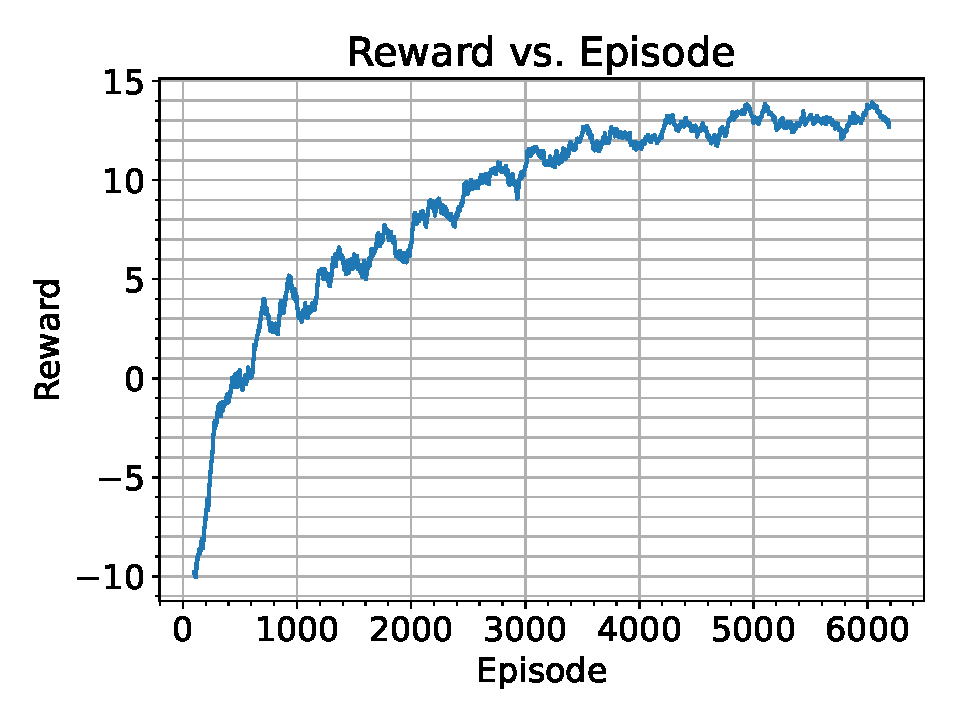
\includegraphics[width=3.4in]{learning_curve}
	\caption{RL reward convergence.}
	\label{fig:learning-curve}
\end{figure}

\subsection{RL model performance}

In order to verify the advantages of an RL-trained drone
in the target visitation mission, we have compared it with
two other baseline agents.
In this comparison, the targets are fixed but their
positions are unknown and based on the distribution
shown in Fig.~\ref{fig:position-distribution}.

The first agent is a drone that completes the same mission 
while moving completely randomly. 
In other words, the probability of taking each of the 
nine available actions is the same.
The second agent moves in a zig-zag manner, as shown
in Fig.~\ref{fig:zigzag}, thus visiting
each cell only once to accomplish the mission.
This pattern may start from the beginning (cell 1) or 
the end (cell 25).
We have included both variants, named Zigzag1 and Zigzag2
respectively, to make the comparison comprehensive.

\begin{figure}[!t]
	\centering
	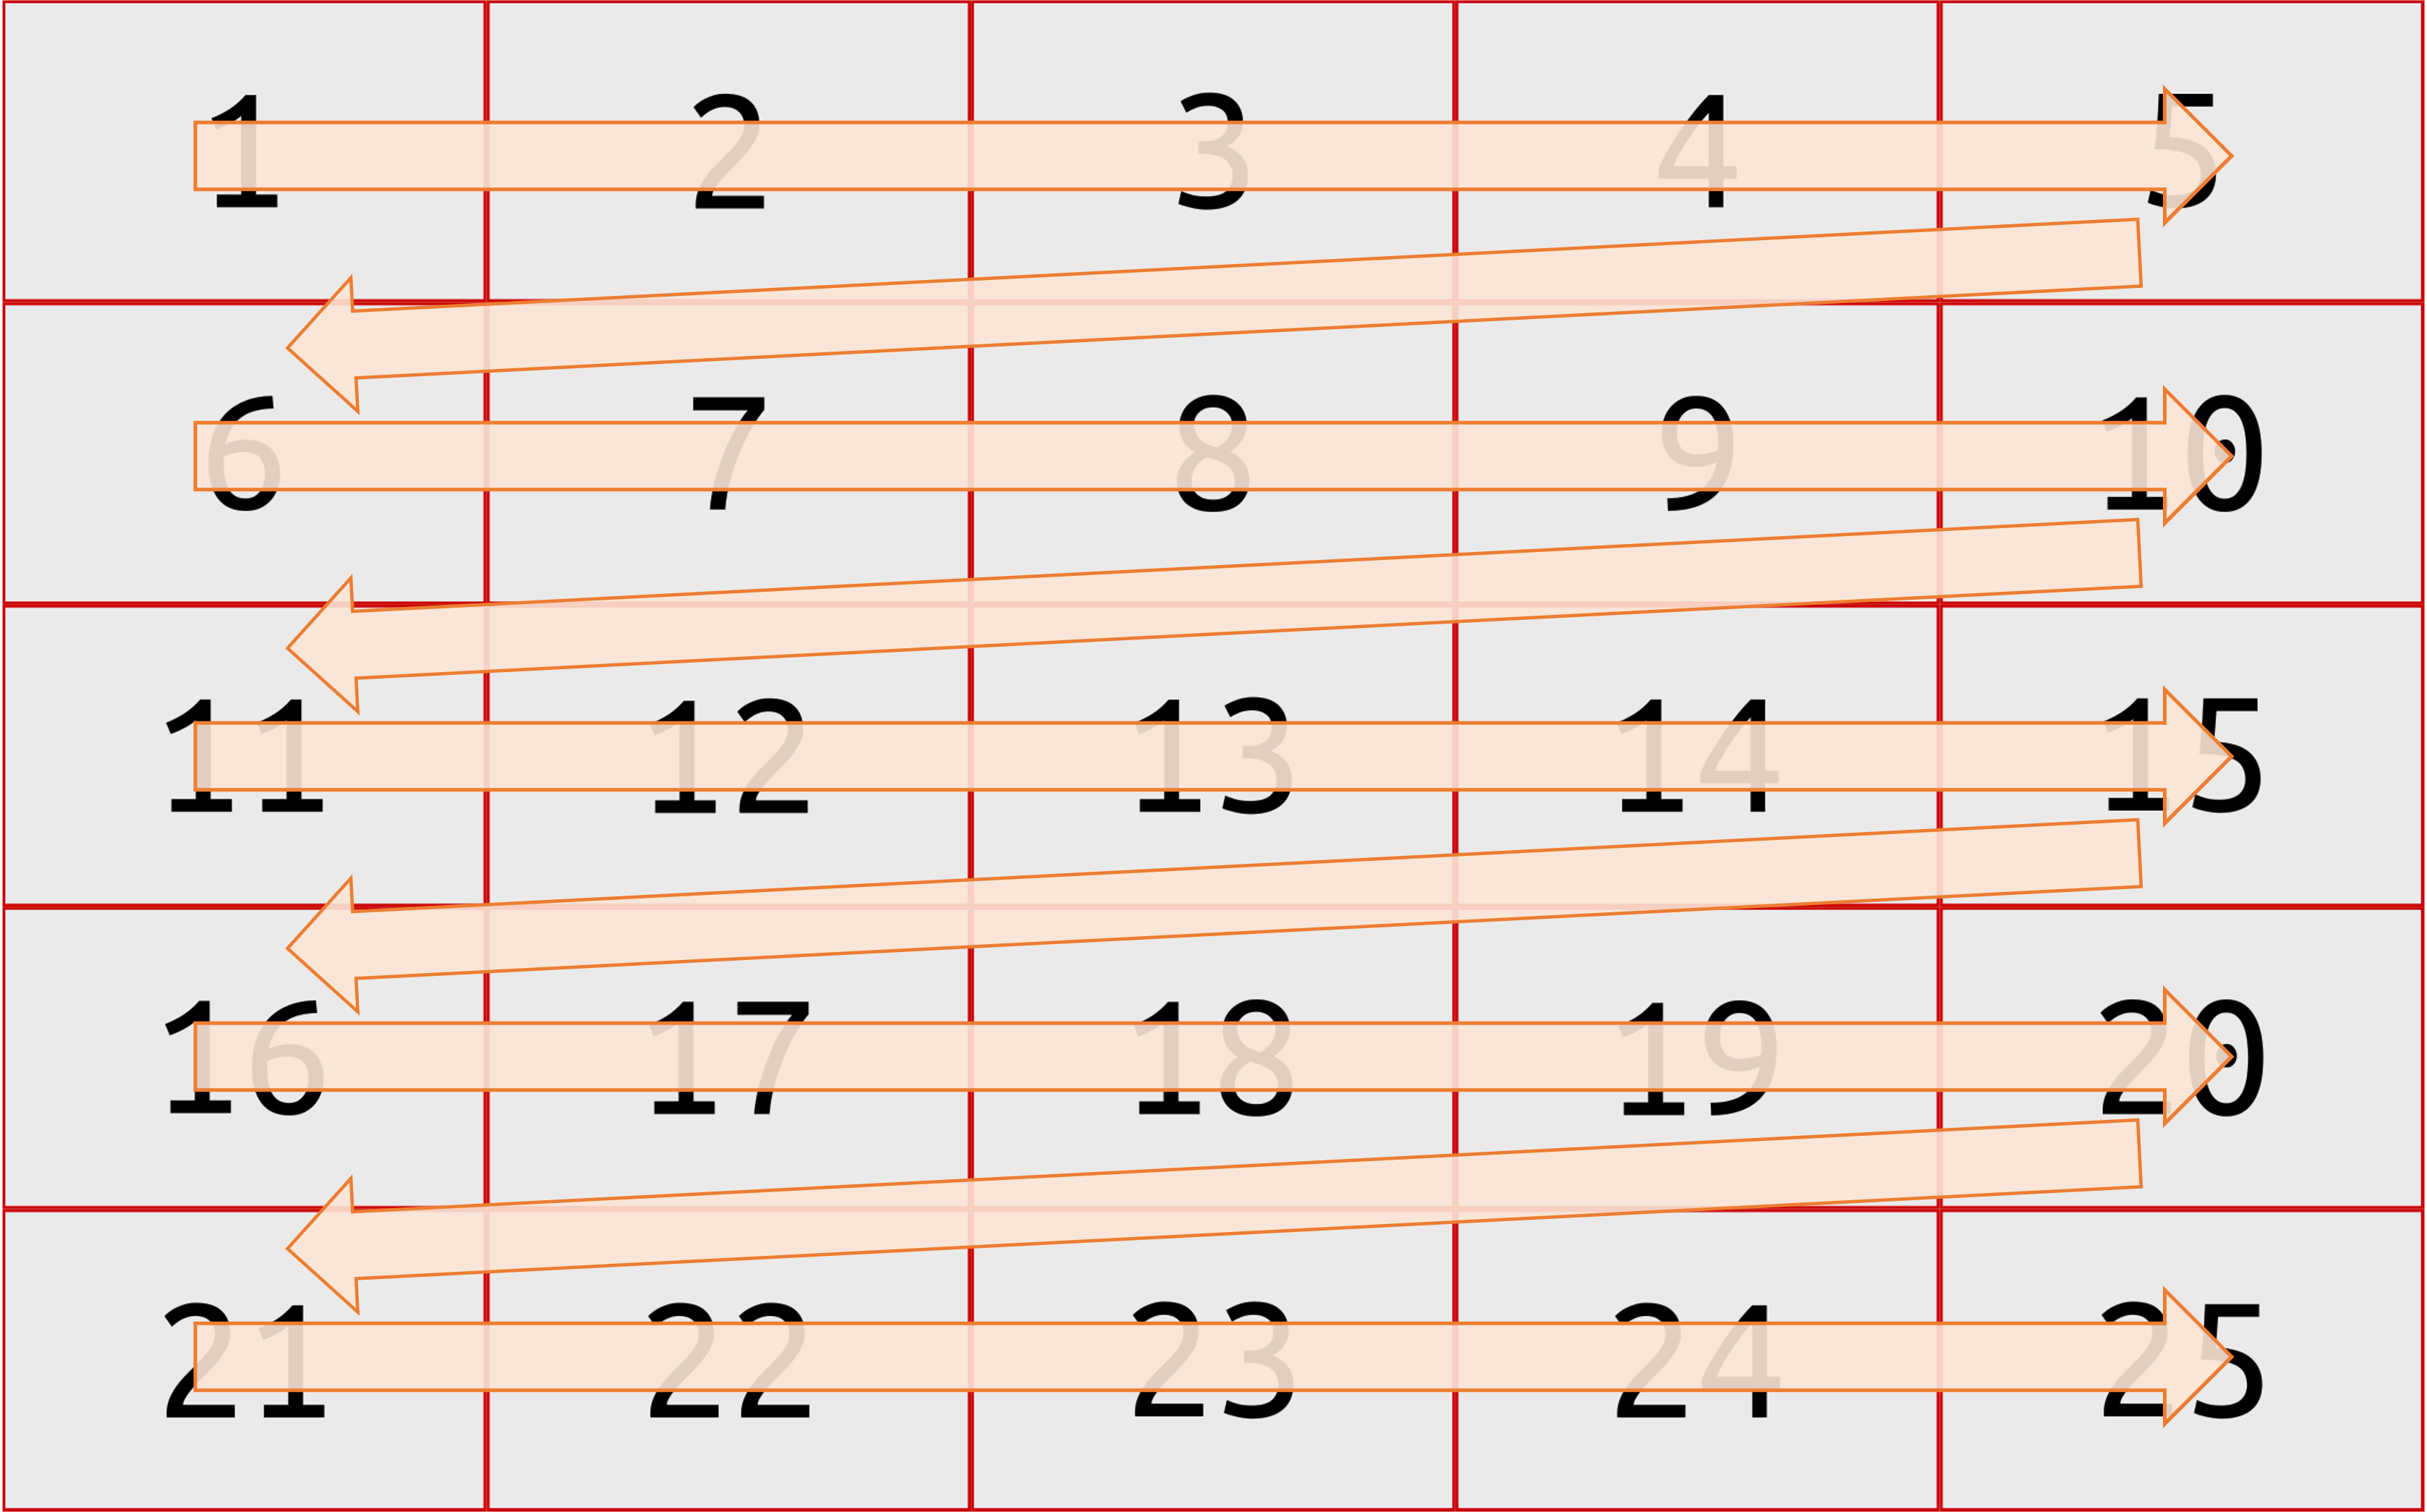
\includegraphics[width=3.4in]{zigzag}
	\caption{The directions of the drone moving zig-zag
		across the grid according to zigzag-1.
                zigzag-2 begins from cell 25.}
	\label{fig:zigzag}
\end{figure}

To make the comparison objective, 
each of the nine actions executed by random, zig-zag
or RL techniques is treated the same way regardless 
of the fluctuations that may arise in the 
distance travelled and speed during
the simulation.
In other words, the distance travelled does not depend
on the technique used but only 
the type of action taken. 
The distances are listed in Table~\ref{tab:distances}.

\begin{table}[!t]
\caption{The distances travelled by each action based on
    the grid 25x40m\textsuperscript{2} shown in 
    Fig.~\ref{fig:grid}.}
\label{tab:distances}
\centering
\begin{tabular}{|p{1.4in}|c|}
\hline
Movement directions & Distances, $d$ (m) \\
\hline
\raggedright Forward-left, forward-right, 
backward-left, backward-right & 9.434 \\
Forward, backward & 5.000 \\
Right, left & 8.000 \\
Starting cell to edge cell e.g. 13\textrightarrow 1 (for zigzag) & 18.868 \\
\raggedright Long diagonal e.g. 5\textrightarrow 6 (for zigzag) & 32.388 \\
\hline
\end{tabular}
\end{table}

On the other hand, the speed is constant for all actions. 
The constant values of speed along with processing time,
and power consumed during movements and hovering
are presented
in Table~\ref{tab:assumptions}
and they are used in the calculations.
Furthermore, since the performance of the agent,
especially the random one, can vary widely and
the positions of the targets are different in each episode, 
10 trials are carried out for each technique and
the average time is taken.

\begin{table}[!t]
\caption{The values assumed to be constant throughout the
mission.}
\label{tab:assumptions}
\centering
\begin{tabular}{|l|c|c|}
\hline
Parameter & Symbol & Value \\
\hline
Speed & $v$ & 5 m/s \\
Processing time & $t_{\text{process}}$ & 1 s \\
Hovering time & $t_{\text{hover}}$ & 2 s \\
Power for moving & $P_{\text{move}}$ & 20 W \\
Power for hovering & $P_{\text{hover}}$ & 10 W \\
\hline
\end{tabular}
\end{table}

Equation~\ref{eq:move-time} shows the formula used to
calculate the time taken for a moving action and
eq.~\ref{eq:hover-time} for a hovering one.
For the energy, moving actions' consumptions are calculated
by eq.~\ref{eq:move-energy} while a hovering one by
eq.~\ref{eq:hover-energy}.
\begin{align}
t_{\text{move,tot}} &= 
\frac{d}{v} + t_{\text{process}}
	\label{eq:move-time}
        \\
t_{\text{hover,tot}} &= 
t_{\text{hover}} + t_{\text{process}}
	\label{eq:hover-time}
        \\
E_{\text{move,tot}} &= 
\frac{d}{v} \cdot P_{\text{move}} 
+ t_{\text{process}} \cdot P_{\text{hover}}
	\label{eq:move-energy}
        \\
E_{\text{hover,tot}} &= 
\left( t_{\text{hover}} + t_{\text{process}} \right) \cdot P_{\text{hover}}
	\label{eq:hover-energy}
\end{align}

The results are presented as bar charts in 
Fig.~\ref{fig:time-plot} and Fig.~\ref{fig:energy-plot}.
Both of the plots indicate that the RL agent completed
the mission in the shortest time and least energy, followed
by the Zigzag2 since it started in an area 
where the probability
distribution of the targets is the highest.
In fact, the RL agent is about twice as fast and twice
as energy-saving as Zigzag2.

The RL performed the best in this environment because
the targets were not placed in a uniform distribution
across the grid,
in which the random agent may have equalled the performance,
neither were they placed deterministically, 
in which case the zig-zag technique with the
right starting point would have won.
Another interesting observation from the comparison is that
the RL agent did not execute the hovering action at all
because after so many timesteps choosing to hover and
receiving a reward of -1, it has learnt that it is an
action that is not beneficial in all states.

\begin{figure}[!t]
	\centering
	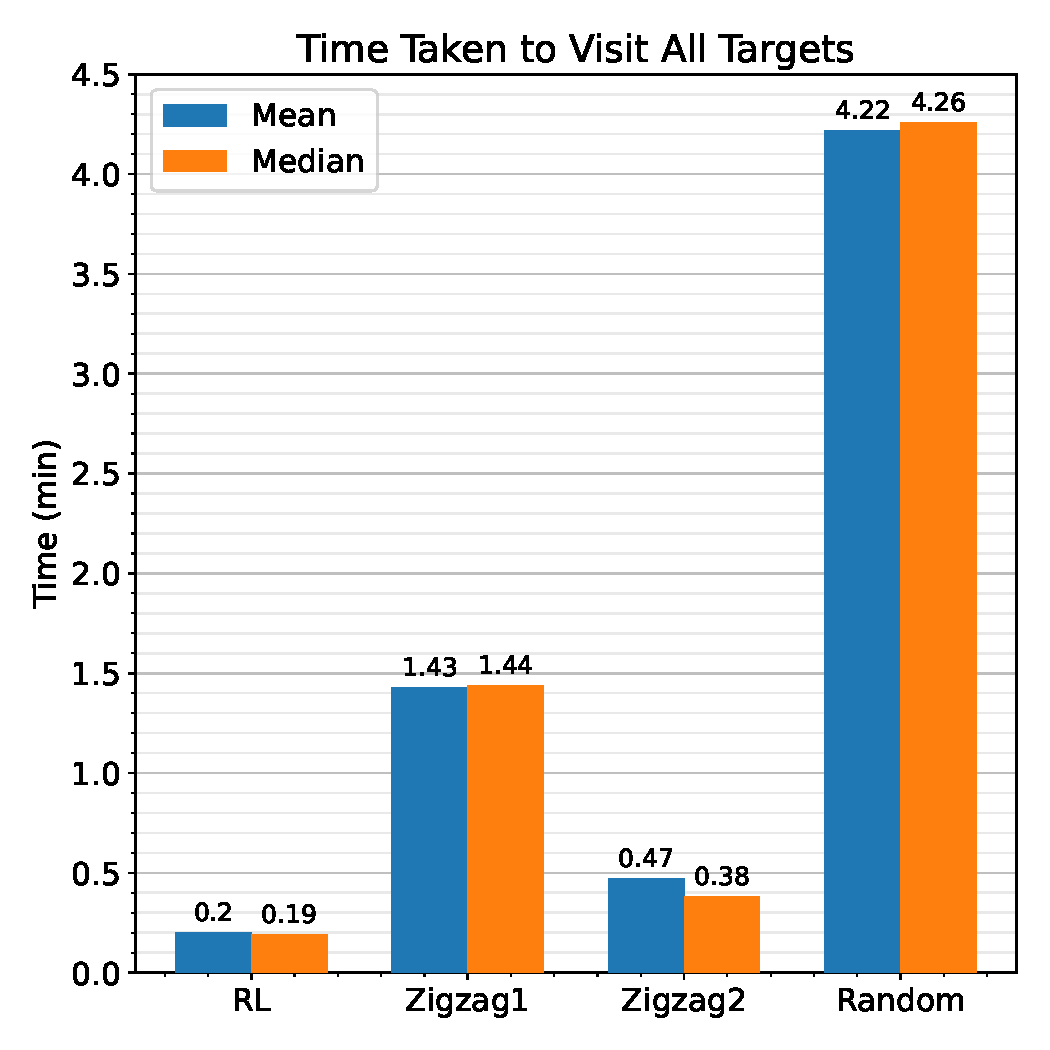
\includegraphics[width=3.4in]{time_plot}
	\caption{The time taken by each technique
        to complete the mission showing the mean,
    median and the quartiles.}
        \label{fig:time-plot}
\end{figure}

\begin{figure}[!t]
	\centering
	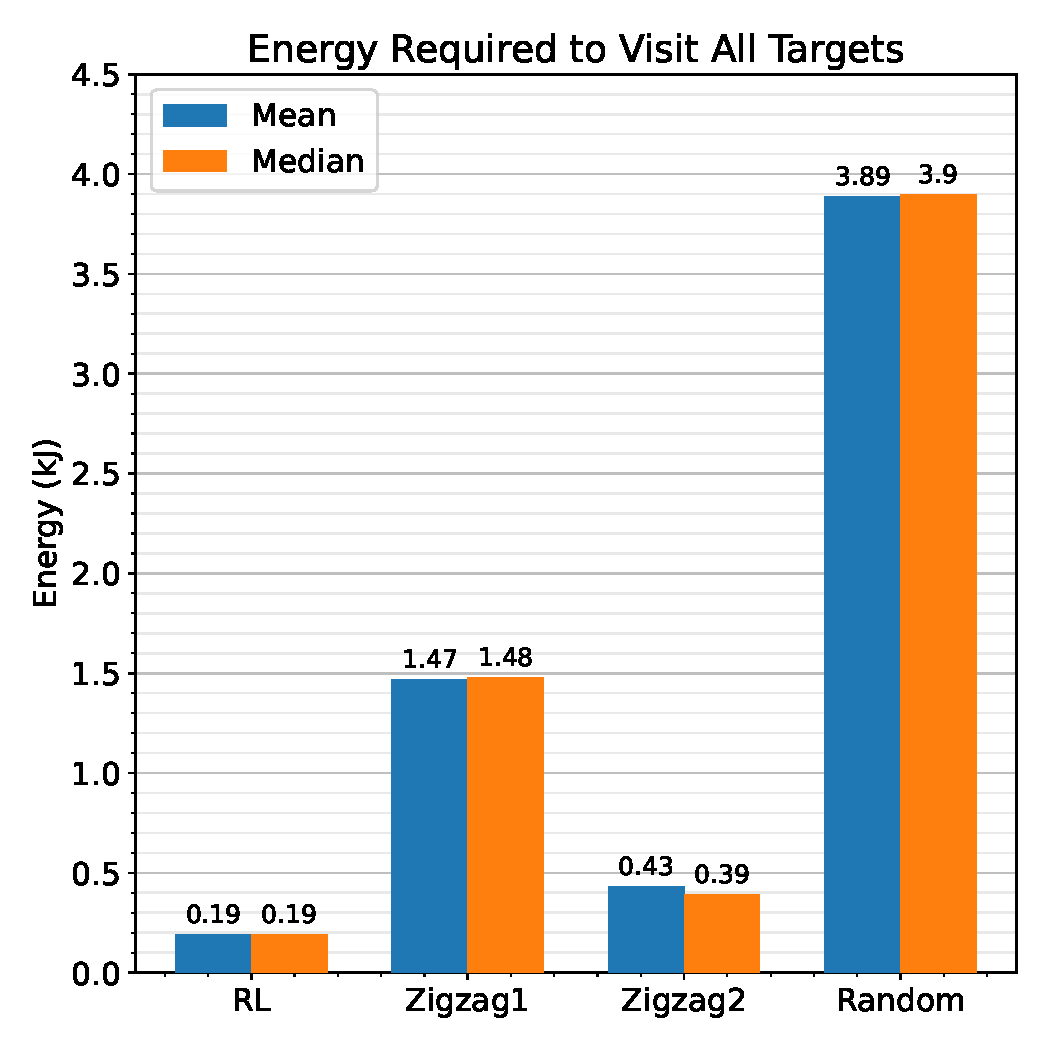
\includegraphics[width=3.4in]{energy_plot}
	\caption{The energy consumed by each technique
        to complete the mission showing the mean,
    median and the quartiles.}
        \label{fig:energy-plot}
\end{figure}

\subsection{User interface}

\lipsum[1]

\end{document}
